% Created by tikzDevice version 0.12
% !TEX encoding = UTF-8 Unicode
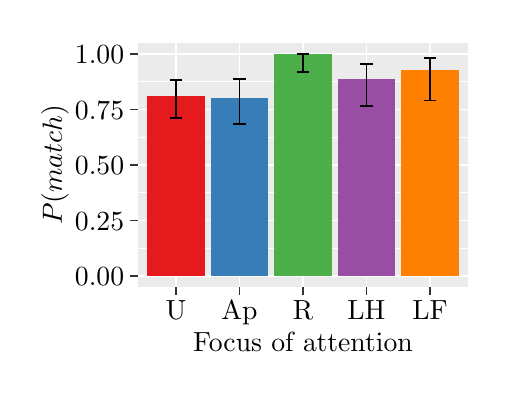
\begin{tikzpicture}[x=1pt,y=1pt]
\definecolor{fillColor}{RGB}{255,255,255}
\path[use as bounding box,fill=fillColor,fill opacity=0.00] (0,0) rectangle (164.64,124.59);
\begin{scope}
\path[clip] (  0.00,  0.00) rectangle (164.64,124.59);
\definecolor{drawColor}{RGB}{255,255,255}
\definecolor{fillColor}{RGB}{255,255,255}

\path[draw=drawColor,line width= 0.6pt,line join=round,line cap=round,fill=fillColor] (  0.00,  0.00) rectangle (164.64,124.59);
\end{scope}
\begin{scope}
\path[clip] ( 39.80, 30.86) rectangle (159.14,119.09);
\definecolor{fillColor}{gray}{0.92}

\path[fill=fillColor] ( 39.80, 30.86) rectangle (159.14,119.09);
\definecolor{drawColor}{RGB}{255,255,255}

\path[draw=drawColor,line width= 0.3pt,line join=round] ( 39.80, 44.90) --
	(159.14, 44.90);

\path[draw=drawColor,line width= 0.3pt,line join=round] ( 39.80, 64.95) --
	(159.14, 64.95);

\path[draw=drawColor,line width= 0.3pt,line join=round] ( 39.80, 85.00) --
	(159.14, 85.00);

\path[draw=drawColor,line width= 0.3pt,line join=round] ( 39.80,105.05) --
	(159.14,105.05);

\path[draw=drawColor,line width= 0.6pt,line join=round] ( 39.80, 34.87) --
	(159.14, 34.87);

\path[draw=drawColor,line width= 0.6pt,line join=round] ( 39.80, 54.92) --
	(159.14, 54.92);

\path[draw=drawColor,line width= 0.6pt,line join=round] ( 39.80, 74.98) --
	(159.14, 74.98);

\path[draw=drawColor,line width= 0.6pt,line join=round] ( 39.80, 95.03) --
	(159.14, 95.03);

\path[draw=drawColor,line width= 0.6pt,line join=round] ( 39.80,115.08) --
	(159.14,115.08);

\path[draw=drawColor,line width= 0.6pt,line join=round] ( 53.57, 30.86) --
	( 53.57,119.09);

\path[draw=drawColor,line width= 0.6pt,line join=round] ( 76.52, 30.86) --
	( 76.52,119.09);

\path[draw=drawColor,line width= 0.6pt,line join=round] ( 99.47, 30.86) --
	( 99.47,119.09);

\path[draw=drawColor,line width= 0.6pt,line join=round] (122.42, 30.86) --
	(122.42,119.09);

\path[draw=drawColor,line width= 0.6pt,line join=round] (145.37, 30.86) --
	(145.37,119.09);
\definecolor{fillColor}{RGB}{228,26,28}

\path[fill=fillColor] ( 43.25, 34.87) rectangle ( 63.90, 99.93);
\definecolor{fillColor}{RGB}{55,126,184}

\path[fill=fillColor] ( 66.20, 34.87) rectangle ( 86.85, 99.28);
\definecolor{fillColor}{RGB}{77,175,74}

\path[fill=fillColor] ( 89.15, 34.87) rectangle (109.80,115.08);
\definecolor{fillColor}{RGB}{152,78,163}

\path[fill=fillColor] (112.09, 34.87) rectangle (132.75,106.17);
\definecolor{fillColor}{RGB}{255,127,0}

\path[fill=fillColor] (135.04, 34.87) rectangle (155.70,109.21);
\definecolor{drawColor}{RGB}{0,0,0}

\path[draw=drawColor,line width= 0.6pt,line join=round] ( 51.28,105.70) --
	( 55.87,105.70);

\path[draw=drawColor,line width= 0.6pt,line join=round] ( 53.57,105.70) --
	( 53.57, 91.98);

\path[draw=drawColor,line width= 0.6pt,line join=round] ( 51.28, 91.98) --
	( 55.87, 91.98);

\path[draw=drawColor,line width= 0.6pt,line join=round] ( 74.23,106.01) --
	( 78.82,106.01);

\path[draw=drawColor,line width= 0.6pt,line join=round] ( 76.52,106.01) --
	( 76.52, 89.67);

\path[draw=drawColor,line width= 0.6pt,line join=round] ( 74.23, 89.67) --
	( 78.82, 89.67);

\path[draw=drawColor,line width= 0.6pt,line join=round] ( 97.18,115.08) --
	(101.77,115.08);

\path[draw=drawColor,line width= 0.6pt,line join=round] ( 99.47,115.08) --
	( 99.47,108.66);

\path[draw=drawColor,line width= 0.6pt,line join=round] ( 97.18,108.66) --
	(101.77,108.66);

\path[draw=drawColor,line width= 0.6pt,line join=round] (120.13,111.39) --
	(124.72,111.39);

\path[draw=drawColor,line width= 0.6pt,line join=round] (122.42,111.39) --
	(122.42, 96.38);

\path[draw=drawColor,line width= 0.6pt,line join=round] (120.13, 96.38) --
	(124.72, 96.38);

\path[draw=drawColor,line width= 0.6pt,line join=round] (143.08,113.55) --
	(147.67,113.55);

\path[draw=drawColor,line width= 0.6pt,line join=round] (145.37,113.55) --
	(145.37, 98.23);

\path[draw=drawColor,line width= 0.6pt,line join=round] (143.08, 98.23) --
	(147.67, 98.23);
\end{scope}
\begin{scope}
\path[clip] (  0.00,  0.00) rectangle (164.64,124.59);
\definecolor{drawColor}{RGB}{0,0,0}

\node[text=drawColor,anchor=base east,inner sep=0pt, outer sep=0pt, scale=  1.00] at ( 34.85, 31.43) {0.00};

\node[text=drawColor,anchor=base east,inner sep=0pt, outer sep=0pt, scale=  1.00] at ( 34.85, 51.48) {0.25};

\node[text=drawColor,anchor=base east,inner sep=0pt, outer sep=0pt, scale=  1.00] at ( 34.85, 71.53) {0.50};

\node[text=drawColor,anchor=base east,inner sep=0pt, outer sep=0pt, scale=  1.00] at ( 34.85, 91.58) {0.75};

\node[text=drawColor,anchor=base east,inner sep=0pt, outer sep=0pt, scale=  1.00] at ( 34.85,111.63) {1.00};
\end{scope}
\begin{scope}
\path[clip] (  0.00,  0.00) rectangle (164.64,124.59);
\definecolor{drawColor}{gray}{0.20}

\path[draw=drawColor,line width= 0.6pt,line join=round] ( 37.05, 34.87) --
	( 39.80, 34.87);

\path[draw=drawColor,line width= 0.6pt,line join=round] ( 37.05, 54.92) --
	( 39.80, 54.92);

\path[draw=drawColor,line width= 0.6pt,line join=round] ( 37.05, 74.98) --
	( 39.80, 74.98);

\path[draw=drawColor,line width= 0.6pt,line join=round] ( 37.05, 95.03) --
	( 39.80, 95.03);

\path[draw=drawColor,line width= 0.6pt,line join=round] ( 37.05,115.08) --
	( 39.80,115.08);
\end{scope}
\begin{scope}
\path[clip] (  0.00,  0.00) rectangle (164.64,124.59);
\definecolor{drawColor}{gray}{0.20}

\path[draw=drawColor,line width= 0.6pt,line join=round] ( 53.57, 28.11) --
	( 53.57, 30.86);

\path[draw=drawColor,line width= 0.6pt,line join=round] ( 76.52, 28.11) --
	( 76.52, 30.86);

\path[draw=drawColor,line width= 0.6pt,line join=round] ( 99.47, 28.11) --
	( 99.47, 30.86);

\path[draw=drawColor,line width= 0.6pt,line join=round] (122.42, 28.11) --
	(122.42, 30.86);

\path[draw=drawColor,line width= 0.6pt,line join=round] (145.37, 28.11) --
	(145.37, 30.86);
\end{scope}
\begin{scope}
\path[clip] (  0.00,  0.00) rectangle (164.64,124.59);
\definecolor{drawColor}{RGB}{0,0,0}

\node[text=drawColor,anchor=base,inner sep=0pt, outer sep=0pt, scale=  1.00] at ( 53.57, 19.03) {U};

\node[text=drawColor,anchor=base,inner sep=0pt, outer sep=0pt, scale=  1.00] at ( 76.52, 19.03) {Ap};

\node[text=drawColor,anchor=base,inner sep=0pt, outer sep=0pt, scale=  1.00] at ( 99.47, 19.03) {R};

\node[text=drawColor,anchor=base,inner sep=0pt, outer sep=0pt, scale=  1.00] at (122.42, 19.03) {LH};

\node[text=drawColor,anchor=base,inner sep=0pt, outer sep=0pt, scale=  1.00] at (145.37, 19.03) {LF};
\end{scope}
\begin{scope}
\path[clip] (  0.00,  0.00) rectangle (164.64,124.59);
\definecolor{drawColor}{RGB}{0,0,0}

\node[text=drawColor,anchor=base,inner sep=0pt, outer sep=0pt, scale=  1.00] at ( 99.47,  7.44) {Focus of attention};
\end{scope}
\begin{scope}
\path[clip] (  0.00,  0.00) rectangle (164.64,124.59);
\definecolor{drawColor}{RGB}{0,0,0}

\node[text=drawColor,rotate= 90.00,anchor=base,inner sep=0pt, outer sep=0pt, scale=  1.00] at ( 12.39, 74.98) {\(P(match)\)};
\end{scope}
\end{tikzpicture}
